\documentclass[12pt]{article}

\usepackage{ceai}
\graphicspath{{../figs/}}

\begin{document}
\doublespacing

\title{CE 488/5588: Applied AI for Engineering\\ \large Topic 17: Agentic AI, Human-in-the-Loop Engineering, and Accountability}
\author{}
\date{}
\maketitle

\begin{ch-box}
Topic 15 explained why large language models became useful for engineering knowledge work. Topic 16 then showed that useful systems are rarely just raw models: they are assembled from prompting, retrieval, tools, and workflow structure. Topic 17 now asks what changes when those pieces become persistent, tool-using, multi-step systems that look increasingly agentic. The technical question is no longer only how to get a better answer. It is how to design workflows in which a system can plan, act, recover, escalate, and remain governable under engineering constraints.
\end{ch-box}

\section*{Learning Objectives}
After completing this chapter, you should be able to:
\begin{itemize}
    \item explain what makes an AI workflow \emph{agentic} rather than merely prompt-based;
    \item distinguish among planning, tool use, memory, and execution in an agentic system;
    \item describe the role of reusable skills, tool interfaces, and orchestration layers in engineering agents;
    \item explain why human-in-the-loop design is central to engineering use of agentic systems;
    \item identify major failure modes of agentic AI, including tool misuse, compounding errors, and misplaced trust; and
    \item explain why accountability, auditability, and governance become more urgent as workflows become more autonomous.
\end{itemize}

\section{From Topic 16 to Topic 17}

Topic 16 introduced first-generation LLM engineering patterns: prompt workflows, retrieval-augmented generation, knowledge-graph construction, and ReAct-style loops. Those systems were already more structured than plain chat, but they were still mostly short-horizon and human-directed. Topic 17 moves to the frontier question: what happens when the same system can persist across steps, call multiple tools, store intermediate state, recover from failures, and continue working toward a goal?

This question matters in engineering because many real tasks are not single-turn tasks. A design review may require reading multiple reports, extracting assumptions, checking standards, comparing versions, writing code, generating a summary, and then handing the result back to a human reviewer. In other words, the useful unit of work is often a \emph{workflow}, not a single response.

\begin{alert-box}
\textbf{Scope decision for this chapter:} Topic 17 focuses on modern agentic workflows, persistent tool use, skills, automated research-style systems, and the human-in-the-loop question. It does not assume that autonomy is automatically desirable. Instead, it studies where autonomy helps, where it fails, and how engineering responsibility changes when systems act in multiple steps.
\end{alert-box}

\section{What Makes a System Agentic?}

The term \textbf{agentic AI} is often used loosely. Not every tool-using model is an agent in the strong sense. A useful working definition is this: a system becomes agentic when it can pursue a goal over multiple steps by combining planning, action, intermediate state, and adaptation to observations.

\begin{def-box}
\textbf{Working definition.} An \textbf{agentic system} is a workflow in which an AI component can select actions, use tools, inspect observations, update its internal plan, and continue toward a goal over multiple steps rather than only producing a single bounded response.
\end{def-box}

This definition highlights four ideas:
\begin{itemize}
    \item \textbf{goal persistence:} the system is trying to complete a task, not merely answer one prompt;
    \item \textbf{action selection:} the system chooses among possible operations such as retrieval, code execution, or delegation;
    \item \textbf{state:} the workflow retains memory of what has already happened; and
    \item \textbf{adaptation:} later actions depend on what earlier steps discovered.
\end{itemize}

\begin{figure}[ht]
    \centering
    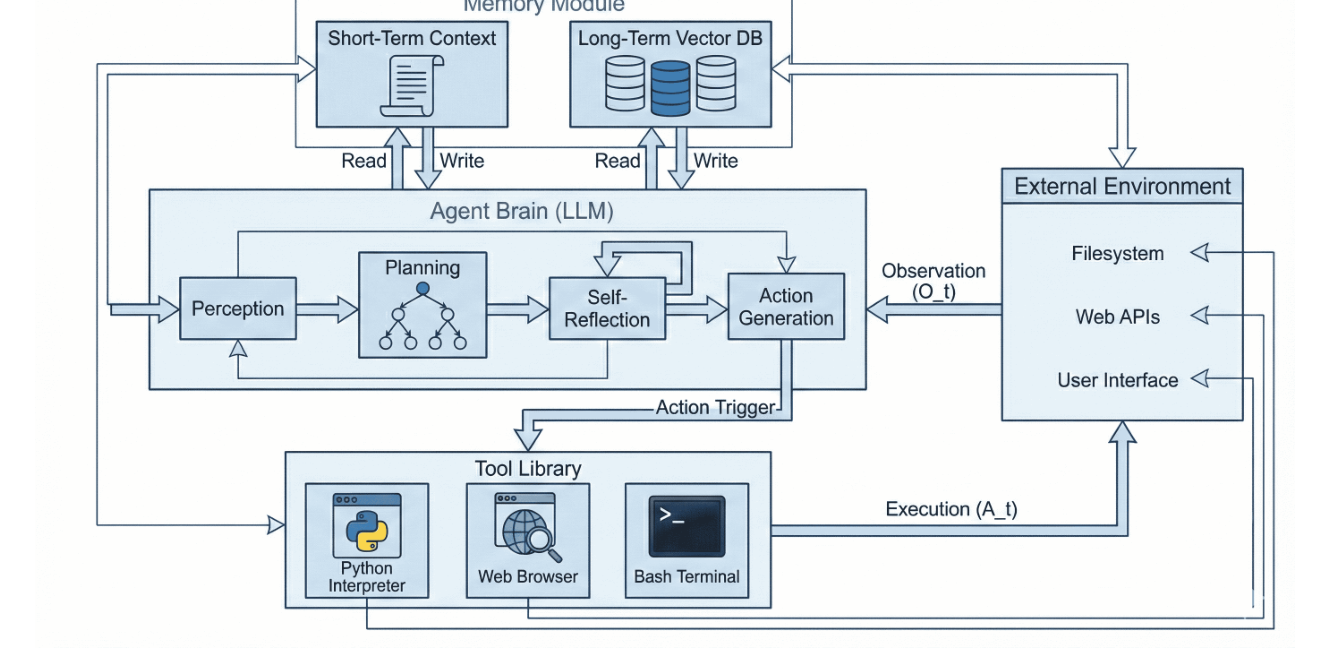
\includegraphics[width=0.92\textwidth]{Topic17fig01.png}
    \caption{Unified architecture of agentic AI. The figure shows how reasoning, memory, tools, and the external environment are organized into a larger agentic workflow. Adapted from Arunkumar, Gangadharan, and Buyya (2026), arXiv:2601.12560, courtesy of the authors under the arXiv nonexclusive distribution license.}
    \label{t17fig:agent_loop}
\end{figure}

Figure~\ref{t17fig:agent_loop} makes clear why Topic 17 goes beyond Topic 16. In Topic 16, the main concern was how one response could be improved by retrieval, prompting, and tools. In Topic 17, the main concern is how those components are organized into a persistent architecture that can coordinate memory, action, and environment-level feedback across many steps.

\begin{ex-box}
\textbf{Why this external figure helps.} The original paper presents both a taxonomy and a unified architecture. For lecture-note purposes, the architecture figure is more useful than a purely abstract loop because it explicitly shows the interaction among the agent brain, memory, tools, and the environment.
\end{ex-box}

\subsection{Agentic Does Not Mean Fully Autonomous}

Students should be careful not to collapse all agentic systems into a single image of a fully independent machine. In practice, there is a spectrum:
\begin{itemize}
    \item \textbf{tool-assisted chat:} the model can retrieve or call one tool but remains tightly user-directed;
    \item \textbf{workflow agents:} the system can complete a bounded multi-step task under explicit constraints;
    \item \textbf{semi-autonomous agents:} the system can pursue subgoals, recover from some failures, and ask for review only at checkpoints; and
    \item \textbf{frontier autonomous systems:} the system can orchestrate larger plans, invoke many tools, and manage longer-horizon tasks with limited oversight.
\end{itemize}

For engineering, this spectrum matters because the right design is often not maximum autonomy. It is the minimum autonomy that yields useful leverage while preserving verification and control.

\section{Core Components of an Agentic Workflow}

Although implementations differ, most agentic systems can be understood as combinations of a few recurring components.

\subsection{Planning}

The first component is \textbf{planning}. A plan decomposes a large task into intermediate steps. In simple systems, this may be just a written checklist. In more advanced systems, planning may involve task trees, dependency graphs, or dynamic revision of subgoals.

Planning matters because many failures of AI systems are actually failures of decomposition. If the system treats a large engineering task as one undifferentiated prompt, it tends to produce fluent but weak output. If it breaks the task into retrieval, comparison, verification, and synthesis steps, the workflow becomes more reliable.

\subsection{Tool Use}

The second component is \textbf{tool use}. Modern agents are rarely useful if they can only generate text. They become more capable when they can call external operations such as:
\begin{itemize}
    \item document search and retrieval;
    \item code execution;
    \item table or spreadsheet parsing;
    \item file inspection;
    \item web search or remote documentation lookup; and
    \item test, build, or simulation commands.
\end{itemize}

Tool use changes the character of the system. The output is no longer only a continuation of text. It becomes part of a larger control process over external artifacts.

\subsection{Memory and State}

The third component is \textbf{memory} or \textbf{state}. A multi-step system must keep track of what has already happened. This may include:
\begin{itemize}
    \item retrieved evidence;
    \item completed subtasks;
    \item unresolved questions;
    \item prior failures and retries; and
    \item task-specific constraints or user preferences.
\end{itemize}

Without state, the system behaves like a sequence of disconnected prompts. With state, it becomes possible to continue a task, recover from interruption, and avoid repeating the same failed action indefinitely.

\subsection{Execution and Recovery}

The fourth component is \textbf{execution with recovery}. Agentic systems need some logic for what happens when a step fails. A robust workflow does not merely continue blindly. It should inspect the failure, attempt a bounded fix, and escalate when uncertainty becomes too high.

This requirement is especially important in engineering because silent failure can be worse than explicit failure. A brittle system that keeps going confidently after the wrong tool call or the wrong document retrieval can create highly plausible but fundamentally unsound outputs.

\begin{figure}[ht]
    \centering
    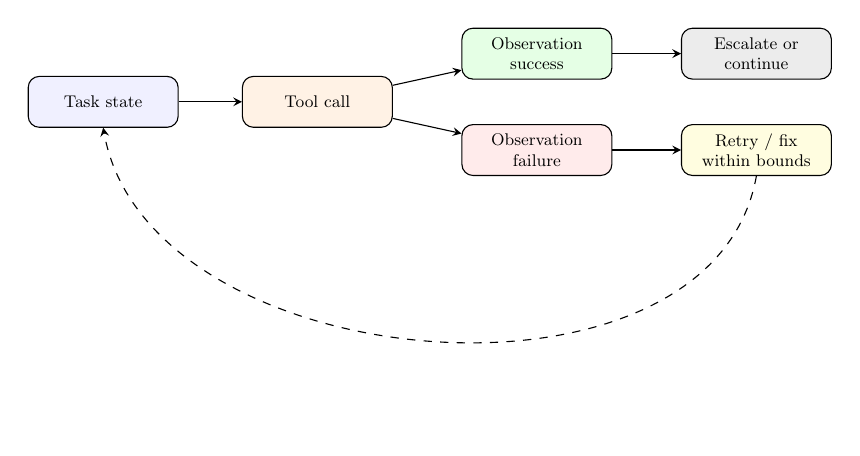
\begin{tikzpicture}[>=stealth,font=\small, scale=0.68, transform shape]
        \tikzset{box/.style={draw, rounded corners, minimum width=2.8cm, minimum height=0.95cm, align=center}}
        \node[box, fill=blue!6] (task) at (0,0) {Task state};
        \node[box, fill=orange!10] (tool) at (4.0,0) {Tool call};
        \node[box, fill=green!10] (ok) at (8.1,0.9) {Observation\\success};
        \node[box, fill=red!8] (fail) at (8.1,-0.9) {Observation\\failure};
        \node[box, fill=yellow!12] (retry) at (12.2,-0.9) {Retry / fix\\within bounds};
        \node[box, fill=gray!15] (human) at (12.2,0.9) {Escalate or\\continue};
        \draw[->] (task) -- (tool);
        \draw[->] (tool) -- (ok);
        \draw[->] (tool) -- (fail);
        \draw[->] (fail) -- (retry);
        \draw[->] (ok) -- (human);
        \draw[dashed,->] (retry.south) to[out=-100,in=-80] (task.south);
    \end{tikzpicture}
    \caption{A simplified execution-and-recovery pattern: inspect outcomes, retry within limits, and escalate when confidence is no longer justified.}
\end{figure}

\section{Skills, Tool Interfaces, and Orchestration}

As agentic workflows become more capable, they are often organized around reusable abstractions. Three of the most useful are \textbf{skills}, \textbf{tool interfaces}, and \textbf{orchestration layers}.

\subsection{Skills as Reusable Task Patterns}

A \textbf{skill} can be understood as a reusable pattern for a class of work. Rather than asking the model to invent a workflow from scratch every time, a skill provides a structured set of instructions, expectations, and tool-use assumptions for a recurring task.

In engineering settings, examples might include:
\begin{itemize}
    \item reviewing a technical manuscript for clarity and consistency;
    \item converting lecture notes into slides;
    \item searching a codebase for architecture patterns;
    \item validating a report against source documents; or
    \item generating a durable handoff for interrupted work.
\end{itemize}

The practical advantage is standardization. Skills reduce the amount of improvisation required from the model and improve consistency across repeated tasks.

\subsection{Tool Interfaces}

A \textbf{tool interface} defines how the system may interact with an external capability. Good tool interfaces matter because they shape what actions are possible, what parameters are explicit, and what outputs can be checked.

For example, a tool that retrieves files, a tool that runs tests, and a tool that performs web search each create different risks and different verification demands. Tool design is therefore not only a software issue. It is also an epistemic issue: what kind of evidence does the tool return, and how much should the agent trust it?

\subsection{Orchestration Layers}

An \textbf{orchestration layer} coordinates the larger workflow. It may decide:
\begin{itemize}
    \item which skill to invoke;
    \item which tool to call next;
    \item whether to continue, retry, or escalate;
    \item how to preserve intermediate state; and
    \item how to route work among specialized subagents or modules.
\end{itemize}

This is one reason frontier AI systems increasingly look like software architectures rather than just models. The model remains central, but the surrounding orchestration determines much of the practical behavior.

\begin{ex-box}
\textbf{Engineering interpretation.} Suppose an organization wants an AI assistant for reviewing bridge-inspection documentation. One skill may summarize field notes; another may compare the notes against prior reports; another may search standards for relevant clauses. The orchestration layer then determines when to call each skill, when to preserve state, and when a human reviewer must intervene before the workflow continues.
\end{ex-box}

\section{Automated Research Assistants}

One visible frontier application of agentic AI is the \textbf{automated research assistant}. This does not mean a system that knows everything. It means a system that can search multiple sources, compare evidence, track subquestions, and produce a structured synthesis over many steps.

In engineering contexts, a research-style assistant may need to:
\begin{itemize}
    \item search official standards, internal reports, and external technical references;
    \item compare several candidate answers to the same question;
    \item track assumptions or unknowns that remain unresolved;
    \item hand results to a human reviewer with citations and caveats; and
    \item keep a record of what was searched, what was found, and what remains uncertain.
\end{itemize}

This is a natural next step beyond Topic 16. The retrieval pipeline from Topic 15 and the system patterns from Topic 16 become subcomponents inside a larger, more autonomous workflow.

\begin{figure}[ht]
    \centering
    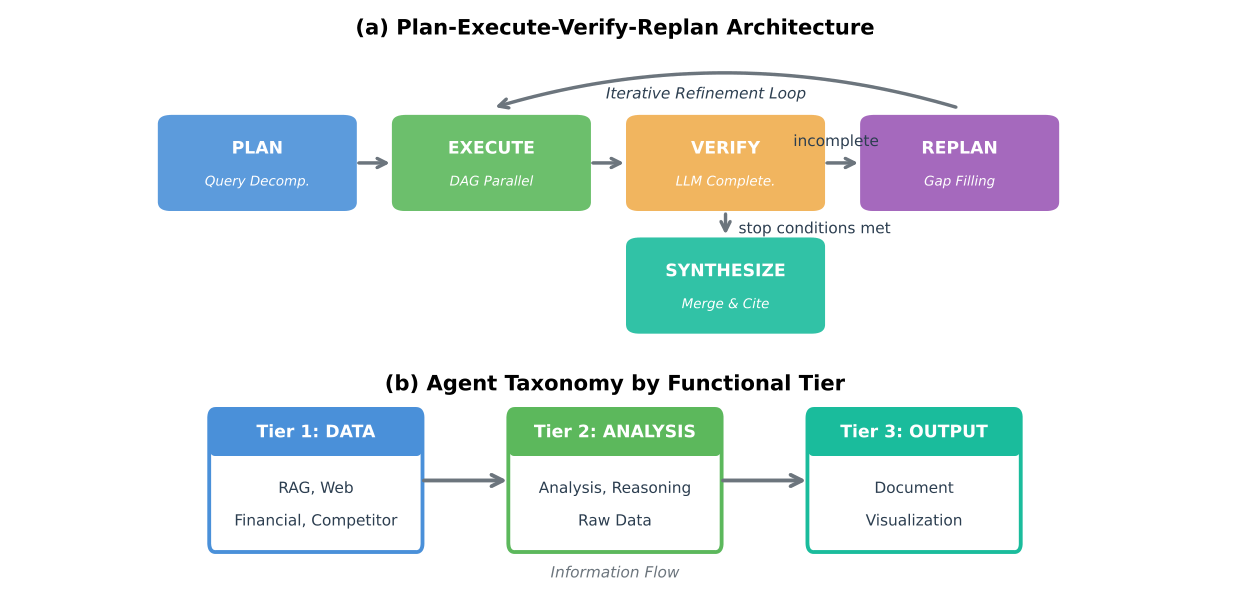
\includegraphics[width=0.92\textwidth]{Topic17fig02.png}
    \caption{Verification-driven multi-agent orchestration. This figure emphasizes a plan-execute-verify-replan structure in which decomposition, parallel execution, and verifier-guided replanning support multi-step question resolution. Adapted from Zhang et al. (2026), arXiv:2603.11445, courtesy of the authors under CC BY-NC-SA 4.0.}
\end{figure}

\subsection{Why This Matters for Engineering}

Engineering work is full of research-like tasks even when the word ``research'' is not used explicitly. A practitioner may need to locate the controlling clause in a standard, inspect prior design assumptions, compare guidance across documents, or justify why one interpretation is safer than another. These are all multi-step tasks with intermediate evidence. A system that can organize those steps can save time, but it can also mislead if it overstates certainty or fails to reveal where the evidence came from.

\begin{ex-box}
\textbf{Why this external figure helps.} The VMAO figure is useful here because it makes the verifier explicit. That matters pedagogically: automated research assistants are not only search-and-summary systems. Their quality depends on how they detect incompleteness, trigger replanning, and decide when the workflow is ready for synthesis or human review.
\end{ex-box}

\section{Human-in-the-Loop Engineering}

The central question of Topic 17 is not whether humans should be removed. It is where humans should remain embedded in the workflow.

\begin{def-box}
\textbf{Human-in-the-loop (HITL).} A \textbf{human-in-the-loop} system is one in which human review, intervention, or approval remains part of the operational workflow rather than being treated as an optional afterthought.
\end{def-box}

In engineering, HITL is not only a convenience. It is often a design requirement because the consequences of error can be physical, legal, financial, or ethical.

\subsection{Where Humans Should Sit in the Loop}

There is no single correct human role for every workflow. Depending on the task, the human may:
\begin{itemize}
    \item specify the objective and constraints at the start;
    \item approve access to tools or external actions;
    \item review intermediate evidence before the system continues;
    \item validate the final result before it is accepted; or
    \item audit the workflow after completion.
\end{itemize}

Different placements of the human correspond to different risk tolerances. High-consequence tasks need earlier checkpoints and more frequent review; lower-consequence tasks can tolerate looser supervision.

\begin{figure}[ht]
    \centering
    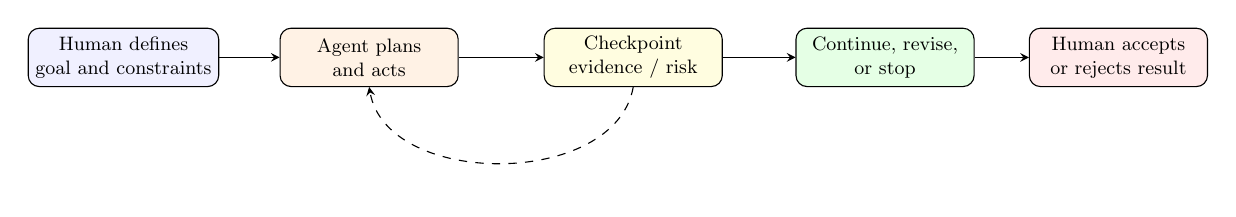
\begin{tikzpicture}[>=stealth,font=\small, scale=0.78, transform shape]
        \tikzset{box/.style={draw, rounded corners, minimum width=2.9cm, minimum height=0.95cm, align=center}}
        \node[box, fill=blue!6] (goal) at (0,0) {Human defines\\goal and constraints};
        \node[box, fill=orange!10] (agent) at (4.0,0) {Agent plans\\and acts};
        \node[box, fill=yellow!12] (checkpoint) at (8.3,0) {Checkpoint\\evidence / risk};
        \node[box, fill=green!10] (revise) at (12.4,0) {Continue, revise,\\or stop};
        \node[box, fill=red!8] (final) at (16.2,0) {Human accepts\\or rejects result};
        \draw[->] (goal) -- (agent);
        \draw[->] (agent) -- (checkpoint);
        \draw[->] (checkpoint) -- (revise);
        \draw[->] (revise) -- (final);
        \draw[dashed,->] (checkpoint.south) to[out=-100,in=-80] (agent.south);
    \end{tikzpicture}
    \caption{A human-in-the-loop control pattern for agentic systems. The human need not micromanage every step, but meaningful checkpoints remain essential when evidence, risk, or uncertainty becomes significant.}
\end{figure}

\subsection{Why HITL Is Not Just a Safety Slogan}

Students should resist hearing ``keep a human in the loop'' as a vague slogan. It is a system-design choice. If the human only sees the final polished output, the loop may be too weak to matter. If the human sees the key evidence, constraints, and decision points, the loop becomes operationally meaningful.

This is why good HITL design depends on more than inserting a final approval step. It requires exposing the right intermediate state, uncertainty, and provenance so that the human can actually exercise judgment.

\section{Failure Modes of Agentic AI}

As systems gain more capabilities, they also gain more ways to fail. Some failures are inherited from ordinary LLMs; others are amplified by multi-step autonomy.

\subsection{Compounding Error}

In a multi-step workflow, one mistake can contaminate later steps. A system that retrieves the wrong standard, misreads a unit, or chooses the wrong file may continue acting on that mistake with increasing confidence. This is one reason multi-step systems can be more dangerous than single-turn systems: the error compounds rather than remaining local.

\subsection{Tool Misuse}

A system may select the wrong tool, pass the wrong parameters, or misinterpret tool output. The more powerful the tool interface, the more consequential this becomes. A wrong search query may waste time; a wrong code edit or wrong external action may change the working state of a project or create a false record.

\subsection{False Escalation and False Non-Escalation}

Another common failure is poor escalation behavior. A system may ask for help too often, making autonomy useless, or ask too rarely, making autonomy reckless. Good engineering workflows therefore need explicit rules for when uncertainty, ambiguity, or risk should trigger human review.

\subsection{Goal Drift}

An agentic system may also drift away from the actual objective. Because it is working over many steps, it may optimize for local completion rather than the true engineering goal. For example, it may produce a polished summary while failing to verify whether the cited source was current or applicable.

\begin{alert-box}
\textbf{Important caution.} Multi-step capability does not automatically create deeper understanding. It can also create longer chains of plausible but misdirected behavior. In engineering, this means that process supervision becomes as important as output inspection.
\end{alert-box}

\section{Trust, Accountability, and Governance}

The more agentic a system becomes, the more the central question shifts from capability to governance. In ordinary chat, the main question may be whether the answer is helpful. In agentic workflows, the questions become broader:
\begin{itemize}
    \item who approved the system's actions;
    \item what evidence the system used;
    \item what logs exist for later audit;
    \item who is responsible when the system fails; and
    \item what should be permitted without human review.
\end{itemize}

\subsection{Auditability and Traceability}

Engineering culture already values documentation, checkability, and traceability. Agentic AI increases the importance of these values rather than reducing them. A useful engineering agent should leave behind a trail of its plan, actions, tool outputs, retrieved evidence, and unresolved uncertainties.

This is not bureaucracy for its own sake. It is the basis on which a human can reconstruct why a conclusion was reached and whether that conclusion deserves trust.

\subsection{Responsibility Cannot Be Delegated to the Model}

No matter how capable a system becomes, accountability for an engineering decision cannot simply be assigned to the model. Responsibility remains with the people and organizations that designed, approved, deployed, and acted on the workflow.

This is one reason the phrase \emph{human-in-the-loop} should be paired with \emph{responsibility-in-the-loop}. If the workflow is arranged so that no human truly understands what happened, then the presence of a nominal reviewer does not meaningfully solve the accountability problem.

\begin{alert-box}
\textbf{Engineering governance principle.} As AI systems gain longer horizons, tool access, and partial autonomy, the burden of auditability and explicit responsibility increases rather than decreases.
\end{alert-box}

\section{Design Principles for Engineering Agentic Systems}

We can now summarize a practical set of design principles for engineering use.

\begin{enumerate}
    \item \textbf{Use bounded autonomy.} Give the system enough freedom to be useful, but not so much freedom that verification disappears.
    \item \textbf{Preserve evidence.} Make retrieved sources, tool outputs, and assumptions visible to the human reviewer.
    \item \textbf{Escalate intentionally.} Define when ambiguity, uncertainty, or consequence should trigger human review.
    \item \textbf{Design for recovery.} Multi-step systems should inspect failures, retry within limits, and stop when confidence is no longer justified.
    \item \textbf{Log the process.} Engineering trust depends not only on the final result but on reconstructing how it was obtained.
    \item \textbf{Keep the human decision right where the risk is.} The more consequential the action, the closer human oversight should be to the critical step.
\end{enumerate}

These principles do not eliminate risk, but they provide a way to reason about where agentic workflows are appropriate and where they are not.

\section{Representative Agentic Systems in Practice}

Before concluding, it is useful to name several systems that make these ideas concrete.

\subsection{Web-Navigation and Research Agents}

One early representative example is \textbf{WebGPT}, which combined a language model with a text-based browser so that the system could search the web, inspect pages, and produce cited answers. Pedagogically, WebGPT matters because it demonstrates a central agentic pattern: the system does not answer only from internal memory. It acts in an external information environment and uses those observations to support later reasoning.

Another useful example is the broader family of \textbf{automated research assistants}. Systems of this type search multiple sources, compare findings, track unresolved uncertainties, and then produce a structured synthesis for human review. The point is not that they replace research judgment. It is that they move some of the search, comparison, and bookkeeping burden into a multi-step workflow.

\subsection{Software Engineering Agents}

Agentic behavior is also visible in software systems such as \textbf{GPT Engineer}, \textbf{MetaGPT}, and newer coding agents that can inspect repositories, propose edits, run checks, and continue across multiple steps. These systems are pedagogically useful because software engineering provides a relatively clear environment for observing planning, tool invocation, retry behavior, and handoff to human review.

For Topic 17, the key lesson is not that one framework is best. It is that software engineering already provides concrete realizations of the agentic pattern: natural-language goals, intermediate planning, external actions, testable artifacts, and explicit verification steps.

\subsection{Frameworks and Architectures}

At the framework level, systems such as \textbf{LangChain}-style agents, \textbf{Toolformer}-style tool-using language models, and classical cognitive architectures such as \textbf{Soar} help students see that agentic behavior can be studied at several layers. Some systems emphasize reusable tool interfaces and orchestration. Others emphasize how the model learns to use tools at all. Still others provide an architecture-level theory of intelligent multi-step behavior.

\begin{alert-box}
\textbf{Practical takeaway.} These examples show that agentic AI is not one product category. It is a family of workflow designs that combine planning, tools, state, and review in different proportions depending on the task and risk level.
\end{alert-box}

\section{Putting the Pieces Together}

Topic 17 can now be summarized in one progression:
\begin{enumerate}
    \item Topic 15 showed how language is represented, retrieved, and used as evidence;
    \item Topic 16 showed how models, prompts, retrieval, and tools become usable systems; and
    \item Topic 17 showed how those systems become agentic once they can plan, act, maintain state, recover, and escalate across multiple steps.
\end{enumerate}

The practical lesson is not that engineering should rush toward full autonomy. It is that the design space has changed. Many useful systems now live between simple chat and full autonomy, and the key challenge is to decide how much agency is appropriate for which task.

\section{What This Chapter Covers and What Comes Next}

This chapter focused on the frontier layer of engineering AI workflows. We began by defining what makes a system agentic and why multi-step persistence matters. We then examined the main components of agentic systems: planning, tool use, memory, and recovery. From there we introduced skills, tool interfaces, and orchestration as reusable structures for building larger workflows. We also studied automated research-style assistants as a representative example of multi-step AI work in practice. Most importantly, we centered the question of human-in-the-loop engineering, showing that autonomy does not eliminate the need for human judgment, traceability, and responsibility. Finally, we examined the failure modes, governance questions, and design principles that become essential as systems gain longer horizons and greater operational freedom.

At this point in the course, both students and instructor are reaching less-charted waters. The current AI frontier appears to be advancing in at least two directions at once. One direction is the continued improvement of \textbf{foundation models}: larger training regimes, new attention and memory mechanisms, more capable post-training, and perhaps deeper paradigm shifts toward ideas now discussed under labels such as \textbf{world models}. The other direction is the rapid growth of \textbf{vertical applications}, where many sectors still contain unmet needs that may be accelerated by retrieval, tool use, and human-in-the-loop workflows even when the underlying models are imperfect.

This dual picture should keep our expectations realistic. Agentic systems and HITL workflows already show signs of accelerating classical engineering tasks, but many technical and social problems remain unresolved. That is not unusual. Revolutionary technologies have always changed economic and social activity unevenly, with both leverage and disruption appearing together. AI, at least before the speculative idea of artificial superintelligence, is not obviously different in that respect. It primarily amplifies human intentions, institutions, and incentives rather than creating new purposes of its own.

Topic 18 will therefore take a broader, more speculative but still fact-based view of the future discussion around AI. We will examine themes that are actively debated in the community: \textbf{neural-symbolic systems} that go beyond current agentic workflows, \textbf{world models}, and the idea of \textbf{ASI}. At the same time, we will revisit the deeper notion of \textbf{embedded intelligence}. If we look at a paramecium or an amoeba---let alone a crow or a dolphin---we are forced to ask whether we even understand how to create genuinely embodied intelligence before speaking confidently about building an AI that surpasses humans in the broadest sense.

The chapter closes with a personal engineering slogan: regardless of the paradigm, engineers stay above AI. We design it, constrain it, audit it, and remain responsible for how it enters the world.

\end{document}
